\documentclass[spanish, fleqn]{article}
\usepackage[english]{babel}
\usepackage[utf8]{inputenc}
\usepackage{amsmath}
\usepackage{amsfonts}
%\usepackage{wasysym}
%\usepackage{mathrsfs}
\usepackage[colorlinks, urlcolor=blue]{hyperref}
\usepackage[top = 2.5cm, bottom = 2cm, left = 2.5cm, right = 2.5cm]{geometry}
\usepackage{fancyhdr, graphicx}
\usepackage{caption}
\usepackage{changepage}
\usepackage{wrapfig}
\usepackage{titling}

\renewcommand{\headrulewidth}{0pt}
\fancyhead[L]{\vbox{
\includegraphics[height=2cm]{Logo_INFO.png} \vspace{0.3cm}}}
\fancyhead[C]{
	\vbox{  \textsc{\large Universidad Técnica Federico Santa María.}\\[0.14cm]
			\textsc{\LARGE Departamento de Informática.} \\[0.14cm]
			\textsc{\Large Sistemas de Gestión, ILI-266.}
			\noindent\makebox[\linewidth]{\rule{18cm}{0.5pt}} }}
\fancyhead[R]{\vbox{
\includegraphics[height=2cm]{Logo_UTFSM.png}\vspace{0.3cm}}}

\title{El programa llamado Organización.} 
\author{Hernán Vargas Leighton -- 201073009-3 \\ hernan.vargas@alumnos.usm.cl}
\date{\today}

\begin{document}
	\maketitle
	\thispagestyle{empty}
	\thispagestyle{fancy}
	\begin{center}
		\begin{minipage}{0.9\textwidth}
			\large \textbf{Resumen:} \\  %no es necesario o si?
			\emph{El presente documento planteará los conceptos 
			básicos por los cuales debemos guiarnos a la hora de mejorar 
			nuestros procesos en busca de la calidad esperada de una empresa 
			desarrolladora de software. En primer lugar se planteará el
			escenario actual para luego explicar cómo se deben aplicar las
			herramientas que éste nos entrega para la gestión de nuestra
			organización.}
			\begin{flushright}
				\textbf{Palabras Clave:} \emph{Mejora Continua, Estandarización,
				Gestión de Calidad.}
			\end{flushright}
		\end{minipage}
	\end{center}
	\section{Introducción.}
	Cuando navegamos por Internet, vemos televisión o leemos el periódico nos
	encontramos constantemente bombardeados de publicidad y en ella
	inequívocamente veremos la palabra calidad a la hora de describir productos
	o servicios, y es que, en el siglo XXI, como nos dice el profesor Osvaldo 
	Ferreira, la calidad ``es un atributo, un estándar básico''\cite{cle1}.
	Pero ¿qué es realmente la calidad? La Real Academia de la Lengua Española
	define calidad en su acepción número uno cómo: ``Propiedad o conjunto de 
	propiedades inherentes a algo, que permiten juzgar su valor''\cite{raecal},
	cómo vemos, al \emph{juzgar un valor} entramos en el terreno de lo subjetivo
	y por ello se hace necesaria una estandarización que nos brinde las bases
	para evaluar la calidad de los productos, procesos, servicios, etc. 
	En este escenario la Organización Internacional de Normalización (ISO del
	griego \emph{isos} que significa \emph{igual}) nos propone diversas normas
	que buscan aunar los esfuerzos a la hora certificar las organizaciones que
	hacen de la búsqueda de la  calidad una parte fundamental de su quehacer.

	El primer documento utilizado como base para la creación de este informe es
	``Normas de calidad: La serie ISO 9000''\cite{cle1} en el cual se nos da 
	una breve introducción a las normas de la serie ISO 9000, que especifican 
	los estándares mínimos a cumplir si buscamos la certificación por dicha 
	institución. La norma ISO 9001 nos guia hacia el mejoramiento continuo y 
	permanente de los procesos, por medio de cuatro pasos que se enuncian de la
	siguiente manera: \emph{``Diga lo que hace'', ``Haga lo que dice'', 
	``Aplique mejoramiento continuo''} y \emph{``Demuéstrelo''}, además se 
	destaca el gran parecido que existen entre estos pasos y el ciclo PDCA 
	(\emph{Plan, Do, Check, Act}). Por último, el documento, nos muestra cómo la
	aplicación del estándar agrega valor a nuestra organización y la hace más
	competitiva.

	El segundo documento analizado es ``Cómo mejorar procesos''\cite{cle2} que
	se centra en una serie de herramientas que nos ayudarán a la hora de
	efectuar el ciclo PDCA en nuestra organización y cómo estás se relacionan 
	entre sí. El gran aporte de estas herramientas radica que ahora las 
	decisiones que se tomen por parte de los directivos de una organización no 
	estarán basadas en la percepción personal o el instinto sino que utilizarán
	el método científico para recabar y analizar la información. 
	Las herramientas utilizadas son: diagramas de flujo, planillas de registro y
	los diagramas de Pareto e  Ishikawa. Todas ellas serán explicadas
	posteriormente.

	El tercer y último artículo analizado tiene por titulo: ``Control 
	estadístico de procesos''\cite{cle3} y nos habla cómo los datos que
	obtenemos gracias al método científico anteriormente descrito no deben ser
	analizados superficialmente. En la mayoría de los procesos productivos se
	recauda información de más de una fuente. La paralelización de las tareas
	hace imposible el análisis de cada rama por separado, por ello debemos 
	recurrir a herramientas estadísticas, en este contexto podemos tener la 
	errónea idea de solo analizar las medias, pensando que las demás variables 
	estadísticas tienen menor relevancia. El artículo nos plantea un método para
	analizar las desviaciones y verificar si nuestros procesos productivos son
	realmente los adecuados.
	\newpage
	\newgeometry{left=2.5cm, right=2.5cm, top=2.5cm, bottom=2.5cm}
	\section{Conceptos básicos.} 
	\begin{wrapfigure}[10]{R}{0.3\textwidth}
		\begin{center}
			\vspace{-0.5cm}
			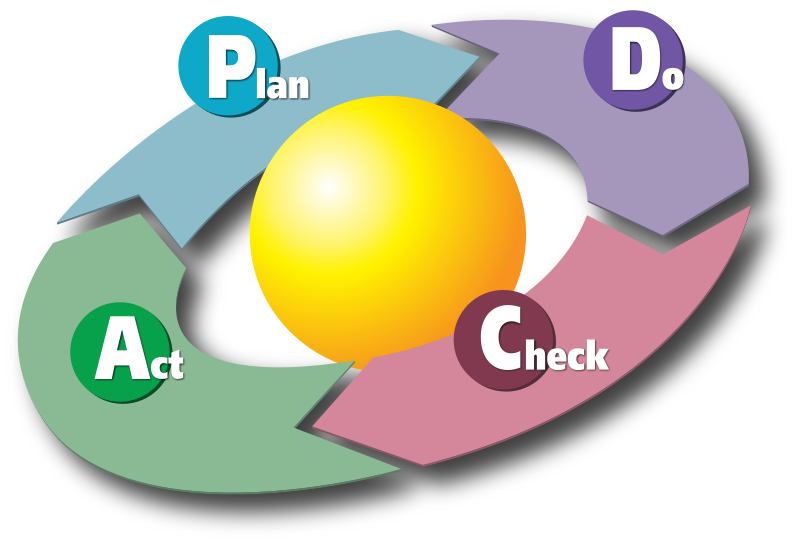
\includegraphics[width=150px]{DPCA.png}
		\end{center}
		Espiral PDCA, con el orden de los pasos.
		Diagram by Karn G. Bulsuk (\url{http://www.bulsuk.com}).
	\end{wrapfigure}
	\textbf{Ciclo PDCA:} O ciclo Deming en honor a su creador, es una
	estrategia de mejora continua que busca mejorar la competitividad
	por medio de un aumento en la calidad, una disminución de costos 
	y una optimización general del proceso. Nos plantea cuatro pasos
	iterativos:
	\begin{enumerate}
		\item
			\textbf{Plan (Planear):} Se establecen y registran las actividades
			que conformarán el proceso y el resultado esperado. 
		\item
			\textbf{Do (Hacer):} Ejecutar el plan establecido, recolectar 
			información del proceso y generar los resultados.
		\item
			\textbf{Check (Verificar):} Con los datos obtenidos del paso
			anterior se hace la comparación con el plan original, se capturan
			las desviaciones y se sacan conclusiones pertinentes.
		\item
			\textbf{Act (Actuar):} También se le llama \textbf{ajustar}, pues
			se toma como base las conclusiones del paso anterior y de ellas se 
			corrigen las desviaciones del plan original, y se extrapolan las
			mejoras a él.
	\end{enumerate}
	\vspace{.25cm}
	\textbf{Diagramas de Flujo:} Son una representación gráfica de un proceso en
	la cual se establecen procedimientos, la relación entre ellos y las 
	interacciones entre el productor y el consumidor. Facilitan la comprensión
	de las etapas, el limite de ellas y ayudan en el conocimiento y 
	entrenamiento.\\[.4cm]
	\textbf{Planillas de Registro:} Es un simple formulario para recopilar 
	datos. A pesar de su simpleza es de vital importancia que estén bien hechos,
	pues serán una de nuestras herramientas fundamentales para la
	retroalimentación. Pueden ser tablas pre-fabricadas para los diferentes
	procesos y deben tener un carácter cuantitativo por sobre cualitativo.\\
	\begin{wrapfigure}[24]{l}{0.6\textwidth}
		\begin{center}
			\vspace{-0.8cm}
			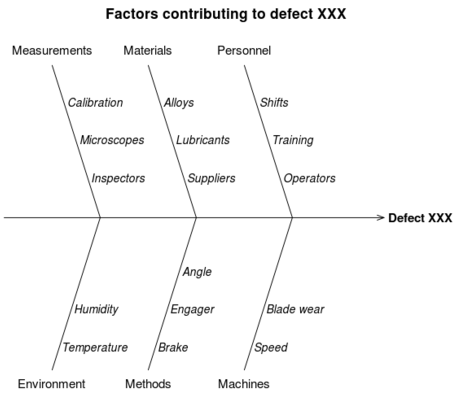
\includegraphics[width=0.6\textwidth]{Ishikawa.png}
		\end{center}
		Ejemplo del diagrama de Ishikawa, por su forma también se le llama
		\emph{espina de pescado}. Imagen creada por Daniel Penfield para 
		Wikipedia. (\url{http://en.wikipedia.org/wiki/File:Cause_and_effect_diagram_for_defect_XXX.svg})
	\end{wrapfigure}
	\textbf{Diagrama de Pareto:} Gráfico de las fallas del proceso, su función
	principal es determinar cuales fallas son más graves que las otras y por
	ello merecen mayor atención y prontitud en su resolución. Tiene un carácter
	cuantitativo y se alimenta de las planillas de registros. El orden en la 
	presentación de los datos es importante, se esperan información sobre los
	porcentajes individuales y el acumulado.\\[.4cm]
	\textbf{Diagrama de Ishikawa:} Método gráfico para identificar posibles 
	causa de defectos en un proceso. Se nutre de los datos recolectados en las
	planillas de registro y se espera que sea desarrollado por integrantes de 
	las diversas áreas de producción, para que así se aporte la mirada de todos
	los segmentos involucrados. La rama principal lleva al defecto, las ramas
	segundarías son las diferentes áreas involucradas en la producción
	defectuosa y las ramas terciarias y superiores son causas y sub-causas del
	error.

	\section{Estándares ISO para la calidad.}
	Como se planteo en la introducción, una buena medida para asegurarnos que 
	nuestros procesos tienen una calidad aceptable es por medio de las
	certificaciones ISO serie 9000, en especifico la ISO 9001 que, como dice su
	pagina web: ``sets out the requirements of a quality management 
	system''\cite{iso9}, es decir: establece los requisitos de un sistema de 
	gestión de calidad. Pero no debemos quedarnos conformes solo con eso, 
	existen estándares que no solo se centran en la calidad del servicio o 
	producto que ofrecemos sino que buscan las características esperadas de las
	organizaciones contemporáneas: gestión ambiental (ISO 14000\cite{iso14}), 
	responsabilidad social (ISO 26000\cite{iso26}) y gestión energética (ISO
	50001\cite{iso501}).
	\subsection{ISO 9000 - Gestión de Calidad.}
	La norma ISO más conocida, provee una guia y herramientas para asegurar en
	gran medida que los productos y servicios ofrecidos satisfacen los
	requerimientos del cliente.
	De la serie 9000 la única certificable es la 9001 que en su versión 2008 se
	implementa en más de un millón de empresas en 170 países\cite{iso9}.
	Consta de 8 principios fundamentales\cite{iso9pdf}:
	\begin{enumerate}
		\item
			\textbf{Enfoque al consumidor:} Toda organización depende de sus 
			clientes, por ello es vital comprender y satisfacer las necesidades
			actuales y futuras de éstos.
		\item
			\textbf{Liderazgo:} El líder debe ser capaz de crear unidad tanto 
			en el propósito como en la dirección de la organización. Es 
			fundamental que todos los miembros se involucren totalmente en el
			cumplimiento de los objetivos.
		\item
			\textbf{Participación:} En todo nivel de la organización es esencial
			el compromiso, de manera que las habilidades de cada uno de los 
			miembros sean utilizadas para el beneficio del conjunto.
		\item
			\textbf{Enfoque basado en procesos:} Cuando las actividades y 
			recursos necesarias para lograr un resultado se tratan gestionan
			cómo un proceso las metas se logran más eficientemente.
		\item
			\textbf{Gestión sistemica:} La eficacia y eficiencia de una 
			organización en el cumplimiento de sus metas generales está 
			determinada por cómo se logran entender, identificar y gestionar
			los procesos interrelacionados como un sistema.
		\item
			\textbf{Mejora continua:} Uno de los objetivos permanentes de la 
			organización es el mejoramiento global del desempeño.
		\item
			\textbf{Deciciones basadas en hechos:} La decisiones efectivas están
			basadas en el análisis de los datos y la información.
		\item
			\textbf{Beneficio mutuo:} Una organización y sus proveedores son 
			ínter-dependientes, una relación mutuamente beneficiosa aumenta
			para ambos la capacidad de generar valor.
	\end{enumerate}
	\subsection{ISO 14000 - Gestión Ambiental.}
	Esta norma aborda diversos aspectos de la gestión del medio ambiente.
	Proporciona herramientas para las organizaciones que buscan identificar y 
	controlar su impacto ambiental. La norma certificable es la 14001 en su
	versión 2004\cite{iso14} aunque no establece requerimientos para un 
	desempeño ambiental aceptable, sino que traza un marco de trabajo por el
	cual las organizaciones pueden hacer eficaz su gestión ambiental y ofrecer
	una garantía a sus empleados de que el impacto ambiental que generan se está
	midiendo y mejorando.\\
	Los beneficios de utilizar la norma incluye:
	\begin{itemize}
		\item Reducción de los costes en la gestión de residuos.
		\item Ahorro en energía y materiales.
		\item Disminución de costos de distribución.
		\item Mejora la imagen corporativa entre clientes y reguladores.
	\end{itemize}
	\subsection{ISO 26000 - Responsabilidad Social.}
	La sociedad es un factor crítico en el operar de una empresa. La ISO 26000
	proporciona orientación sobre cómo operan las empresas socialmente 
	responsables. Esto significa actuar de manera ética y transparente y 
	contribuir a la salud y bienestar de la sociedad.\\
	La norma ISO 26000 en su versión 2010\cite{iso26} proporciona orientación en
	vez de requisitos, por lo cual no es posible certificarse. Fue creada el
	2010 con la participación de organizaciones, representantes del gobierno,
	grupos de consumidores y trabajadores de todo el mundo, por lo que tiene un
	carácter internacional.
	\subsection{ISO 50001 - Gestión Energética.}
	El uso eficiente de la energía no solo reduce considerablemente los costos
	de una organización sino que además ayuda a conservar recursos y hacer 
	frente al cambio climático.\\
	La norma ISO 50001 en su versión 2011\cite{iso501} se basa en aplicar un 
	modelo de mejora continua (como las normas 9001 y 14001) en la gestión 
	energética, lo que hace que sea más fácil para las organizaciones integrar
	ésta en los esfuerzos generales para mejorar la calidad y gestión ambiental.
	\\ La ISO 15001 requiere que las organizaciones:
	\begin{itemize}
		\item Desarrollen una política para el uso eficiente de la energía.
		\item Establezcan metas y objetivos para cumplir dicha política.
		\item Recolecten y utilicen datos para tomar decisiones afines.
		\item Midan los resultados obtenidos.
		\item Revisen cuan bien funciona la política actual.
		\item Mejoren dicha política.
	\end{itemize}

	\section{Desarrollo.}
	Como ingenieros informáticos debemos ser conciertes del escenario
	actual y futuro al que deberán enfrentarse las organizaciones de las que
	posiblemente seremos parte. Las herramientas entregadas, la estrategia de 
	mejora continua y las normas ISO no son ajenas a nuestro rubro y en esta
	sección del documentos me enfocaré en aplicar dichos tópicos a lo que sería
	una empresa de desarrollo de software propiamente tal. En primer lugar se 
	explicará cómo afectan particularmente los estándares ISO a éste tipo de
	organizaciones para luego dar lugar al mejoramiento continuo y por último 
	la aplicación de las herramientas para lograr estás metas.
	\subsection{Estándares ISO}
	La norma ISO 9001 es básica en toda organización, ya sea seamos parte del
	equipo directivo o desarrolladores netos estaremos ligados a ella. En este
	punto es importante notar cómo su enfoque iterativo y búsqueda de 
	satisfacción del cliente es muy similar a lo que se hace generalmente en 
	los modelos de desarrollo en espiral o incremental, lo que me hace suponer
	que apoyará el sistema natural de un equipo de desarrollo.\\
	Las normas ISO 14000 y 26000 no significarán mayor esfuerzo para éste tipo
	de organizaciones, ya que, como el producto final es virtual, y 
	generalmente no se utilizar muchos insumos a la hora de la producción además
	de la creatividad y el tiempo, se esperaría que los desechos generados sean
	menores y el impacto hacia la sociedad sea positivo.\\
	Por último, la ISO 50001 es posiblemente la que mayor repercusión tendrá en
	este tipo de organización, ya que, al trabajar con tecnología dependiente de
	la electricidad, estamos completamente ligados al gasto energético. 
	Recordemos que los datacenter son uno de los pesos pesados a la hora del 
	conteo global del gasto energético\cite{energ} y sin lugar a dudas está es
	una problemática en la cual una empresa de desarrollo de software debe 
	poner sus esfuerzos en solventar.

	\subsection{Mejoramiento continuo.}
	El proceso productivo principal de una empresa de desarrollo de software es
	la creación misma del software, para ello generalmente se desglosa el
	requerimiento inicial del cliente en una serie de módulos con funciones 
	especificas y responsables determinados. En general, en los métodos de 
	desarrollo iterativos, el mejoramiento continuo de éstos módulos está 
	incluido, pero cuando éste se completa no es necesario seguir con él. En
	estos modelos si queremos mejorar nuestro producto es debemos agregar más
	funciones y por ello módulos, pero esto no es necesariamente
	lo que nuestros clientes quieren. Por estas razones considero que para
	los desarrolladores, el mejoramiento está en la distribución del trabajo, 
	la toma de requerimientos, la especialización y el trabajo en equipo.\\
	Desde esta perspectiva el mejoramiento continuo es la labor de aprendizaje
	por la cual los miembros de la organización se hacen cada vez más eficientes
	en sus respectivas áreas. Por ello es fundamental que el ciclo PDCA esté
	enfocado en los factores previamente descritos. Así la gestión del personal
	es fundamental en este tipo de organizaciones, pues ellos son íntegramente
	quienes crean nuestros productos finales.

	\subsection{Utilización de herramientas.}
	Los diagramas de flujo son una herramienta a la cual estamos bastante 
	acostumbrados, los utilizamos para plantear cómo se relacionan los módulos
	o clases de nuestros programas y bases de datos, ahora simplemente debemos
	utilizarlos para modelarnos nosotros mismos en un programa más grande 
	llamado organización.\\
	Las planillas de registros pueden ser mejoradas gracias a nuestros 
	conocimientos informáticos. Se pueden crear planillas virtuales que 
	recolecten la información recogida por muchos funcionarios o incluso
	obtengan información por ellas mismas. Además podemos crear los diagramas
	de Pareto de manera automática gracias a los datos recogidos. Un sistema 
	de gestión virtual con la capacidad de ofrecernos las acciones anteriormente
	descritas será de suma importancia para analizar nuestros ciclos PDCA y 
	puede ser construido por nosotros mismos a la medida de nuestra empresa.\\
	Por último, el diagrama de Ishikawa puede ser utilizado para probar tanto 
	nuestros procedimientos a la hora de crear software como el producto mismo.
	Si vemos el defecto como un \emph{bug} y los departamentos de la empresa
	como lo módulos de nuestro programa, podremos identificar las causas de la
	misma manera en que las encontramos normalmente.

	\section{Conclusiones.}
	El desarrollo de un programa es una lucha constante por crear un sistema 
	perfecto para el propósito que fue pensado. Contamos con diferentes 
	herramientas para ello, como son los modelos de desarrollo, los diagramas
	de clases o bases de datos, los \texttt{debugger}, etc. Ahora, ¿qué tiene
	que ver todo esto con las ideas planteadas en este informe? Creo que, a
	cierto nivel de abstracción son lo mismo: Cuando gestionamos una empresa en
	búsqueda de certificación y calidad lo que hacemos es ser los 
	desarrolladores de este gran programa llamado organización. Utilizamos un
	modelo iterativo para crear nuestros módulos (gestionamos nuestros
	procedimientos con PDCA), nos valemos del UML para crear nuestros diagramas
	de clases (Diagramas de Fujo), generamos una base de datos donde guardar
	toda la información relevante para el correcto funcionamiento del programa
	(planillas de registros) y en ella programamos \texttt{triggers} para 
	notificarnos los errores que vallan sucediendo (diagrama de Pareto) y si
	algo falla utilizamos el \texttt{debugger} para encontrar la causa 
	(diagrama de Ishikawa).\\
	Los estándares, por otra parte, son parte de los requerimientos: la 
	estabilidad y fiabilidad (ISO 9001), el uso de recursos computacionales 
	limitados (ISO 14000 y 50001) y que sea fácil de usar y agradable para
	el consumidor (ISO 26000).\\
	Con todas estas similitudes, la labor de gestión es ideal para un
	informático, pues conocemos cómo funcionan los sistemas, cuales son los
	factores que debemos tomar en cuenta y cómo reaccionar ante las 
	desviaciones que estos presentan.

	\renewcommand{\refname}{\selectfont 6 \, Referencias.} % Hack para nombre
	\begin{thebibliography}{x}
		\bibitem{cle1}
			\textit{Normas de calidad: La serie ISO 9000} - La clase ejecutiva, 
			El Mercurio 4 de abril del 2013, Osvaldo Ferreira Ph.D Universidad 
			de Wisconsin.
		\bibitem{cle2}
			\textit{Cómo mejorar procesos} - La clase ejecutiva, El Mercurio 11
			de abril del 2013, Osvaldo Ferreira Ph.D Universidad de Wisconsin.
		\bibitem{cle3}
			\textit{Control estadístico de procesos.} - La clase ejecutiva, El
			Mercurio 18 de abril del 2013, Osvaldo Ferreira Ph.D Universidad de
			Wisconsin.
		\bibitem{raecal}
			\textit{Definición: Calidad.} - Real Academia Española, Diccionario
			Usual, \url{http://buscon.rae.es/drae/srv/search?val=calidad} 
			revisado el 19 de noviembre del 2014.
		\bibitem{iso9}
			\textit{ISO 9000 - Quality management} - ISO.org, \url{http://www.iso.org/iso/home/standards/management-standards/iso_9000.htm} 
			revisado el 19 de noviembre del 2014.
		\bibitem{iso14}
			\textit{ISO 14000 - Environmental management} - ISO.org, 
			\url{http://www.iso.org/iso/home/standards/management-standards/iso14000.htm}
			revisado el 19 de noviembre del 2014.
		\bibitem{iso26}
			\textit{ISO 26000 - Social responsibility} - ISO.org, 
			\url{http://www.iso.org/iso/home/standards/iso26000.htm}
			revisado el 19 de noviembre del 2014.
		\bibitem{iso501}
			\textit{ISO 50001 - Energy management} - ISO.org, 
			\url{http://www.iso.org/iso/home/standards/management-standards/iso50001.htm}
			revisado el 19 de noviembre del 2014.
		\bibitem{iso9pdf}
			\textit{Quality management principles} - ISO.org, \url{http://www.iso.org/iso/qmp_2012.pdf}
			revisado el 19 de noviembre del 2014.
		\bibitem{energ}
			\textit{Power, Pollution and the Internet} - The New York Times,
			Technology, 
			\url{http://www.nytimes.com/2012/09/23/technology/data-centers-waste-vast-amounts-of-energy-belying-industry-image.html}
			revisado el 19 de noviembre del 2014.
	\end{thebibliography}

	%Referencias.
	\begin{flushright}
		\begin{flalign*}
			&&\text{\textbf{Tiempo SCT}: 
					\emph{Análisis de los artículos}} &= 1:00 \\
				  &&\emph{Investigación} &= 2:15 \\
				  &&\emph{Creación del informe} &= 3:20 \\
				  &&\text{Total} &= 6:35
		\end{flalign*}
	\end{flushright}

\end{document}
